\documentclass[tikz]{standalone}
\usepackage{tikz}
\usetikzlibrary{positioning, graphs}
\usetikzlibrary{graphs.standard}
\begin{document}
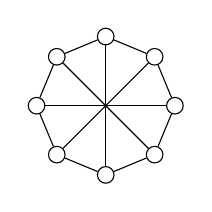
\begin{tikzpicture}
		[every node/.style={draw,circle,inner sep = 0mm, minimum size = 0.6em}]
		\graph[clockwise, radius = 2.5em, empty nodes]{subgraph C_n[n = 8, name = A]};
		
		\foreach \i [evaluate={\j=int(mod(\i+3,8)+1)};] in {1, 2, 3, 4}{
			\draw (A \i) -- (A \j);
		}
\end{tikzpicture}
\end{document}